\chapter{実環境における配管設備での検証実験}
本章では、RGB画像ベースおよびRGB-D画像ベースの6D姿勢推定を用いた配管のアイソメ図生成の有効性を検証するため、実環境における配管設備での検証実験を行った。

\section{実験方法}
本実験の実施において、まずデータ収集を行った。
配管画像の取得には、Microsoft社製のRGB-Dカメラ「Azure Kinect DK」を使用した。
次に、第2章で述べた深層学習を用いた6D姿勢推定手法について、RGB画像ベースおよびRGB-D画像ベースの2つの方法を用いて検証を行った。
最後に、両手法を用いて配管のアイソメ図を生成し、その精度について評価を実施した。

\section{RGB画像に基づく6D姿勢推定のデータセット収集}

\subsection{物体検出}
物体検出に使用したYOLOにおけるデータセットの収集について説明する。
深層学習による認識ネットワークにはデータセットの数量が多いほど精度とロバスト性が向上する。
それは様々な場面での配管の写真を学習することによってどの環境においても対応できる汎用性が高まることを意味している.
物体検出のデータセットには、画像内の配管の曲管とT字管の接続部の位置をバウンディングボックスによって、ラベル付けを行うことでデータセットを作成した。
物体検出のラベリングの例を図\ref{fig:f1}に示す。
\begin{figure}[htbt]
	\centering
	 \includegraphics[height=55mm]{Figure/label_detection.eps}
	 \caption{物体検出のラベリングの例}
	 \label{fig:f1}
\end{figure}

\subsection{画像マッチング}
続いて、Gen6Dの画像マッチングに使用する参照画像のデータセットについて説明する。
まず、T字管および曲管を周囲から撮影した動画を収集し、各動画から10フレームごとに1枚の画像をサンプリングし、約200枚の参照画像を取得した。
本検証で用いたT字管の参照画像の一部の例を図\ref{fig:f2}に示す。
\begin{figure}[htbt]
  \centering
   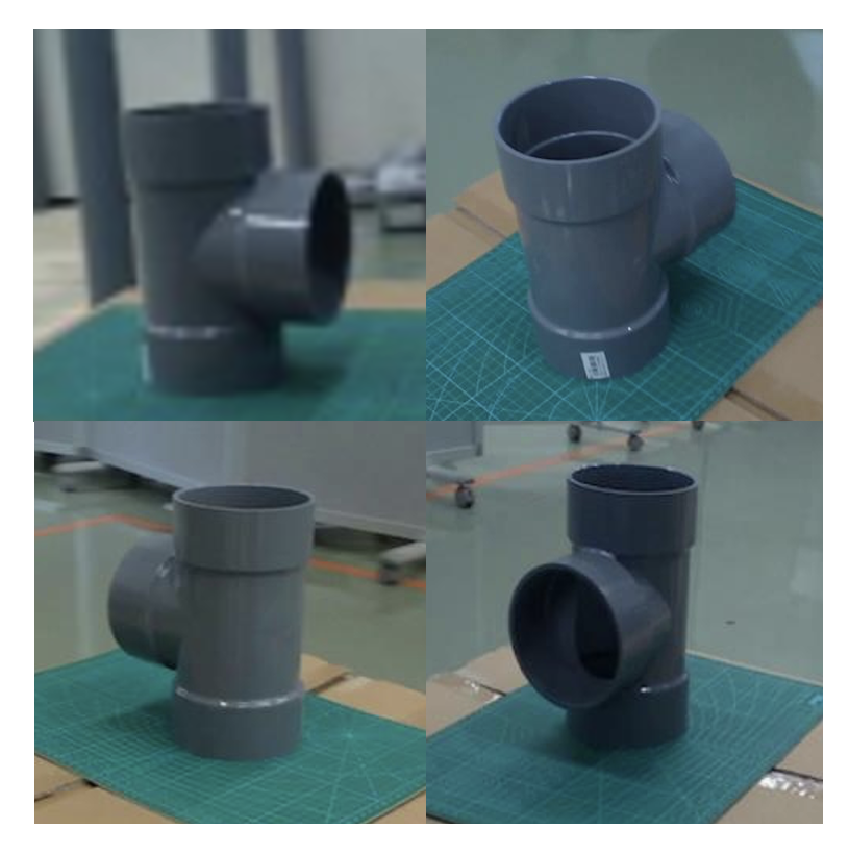
\includegraphics[height=95mm]{Figure/ref_images.eps}
   \caption{参照画像の例}
   \label{fig:f2}
\end{figure}

参照画像の3次元点群データを取得するために、Structure from Motion(SfM)手法を用いるColmapソフトウェアを使用した。
Colmapは、異なる視点から撮影した複数の2D画像を基に3D点群を再構築するソフトウェアである。
各動画シーケンスに対して、Colmapを用いてカメラの外部および内部パラメータを復元した。
また、Colmapを用いて得られた3D点群データを図\ref{fig:f3}に示す。
\begin{figure}[htbt]
  \centering
   \includegraphics[height=95mm]{Figure/colmap.eps}
   \caption{Colmapを用いた3D点群データ}
   \label{fig:f3}
\end{figure}


\section{RGB-D画像に基づく6D姿勢推定のデータセット収集}
\subsection{インスタンスセグメンテーション}
RGB-D画像を用いた配管6D姿勢推定に用いたSAM-6Dによるインスタンスセグメンテーションに用いたデータセットの紹介をする。
インスタンスセグメンテーションのデータセットには、RGB画像内の配管の曲管とT字管の接続部の位置をピクセル単位でマスク化した。
インスタンスセグメンテーションのラベリングの例を図\ref{fig:f4}に示す。
\begin{figure}[htbt]
	\centering
	 \includegraphics[height=55mm]{Figure/label_segment.eps}
	 \caption{インスタンスセグメンテーションのラベリングの例}
	 \label{fig:f4}
\end{figure}

\subsection{ポイントマッチング}
SAM-6Dで用いたポイントマッチングに用いたデータセットの紹介をする。

検出クラスであるT字管および曲管の3Dモデルを利用してテンプレート画像を生成する。
テンプレート画像は、3DソフトウェアであるBlenderを使用して、対象物を中心に配置されたカメラからさまざまな角度のビューを取得する。
テンプレート画像の例を図\ref{fig:f5}に示す。
\begin{figure}[htbt]
  \centering
   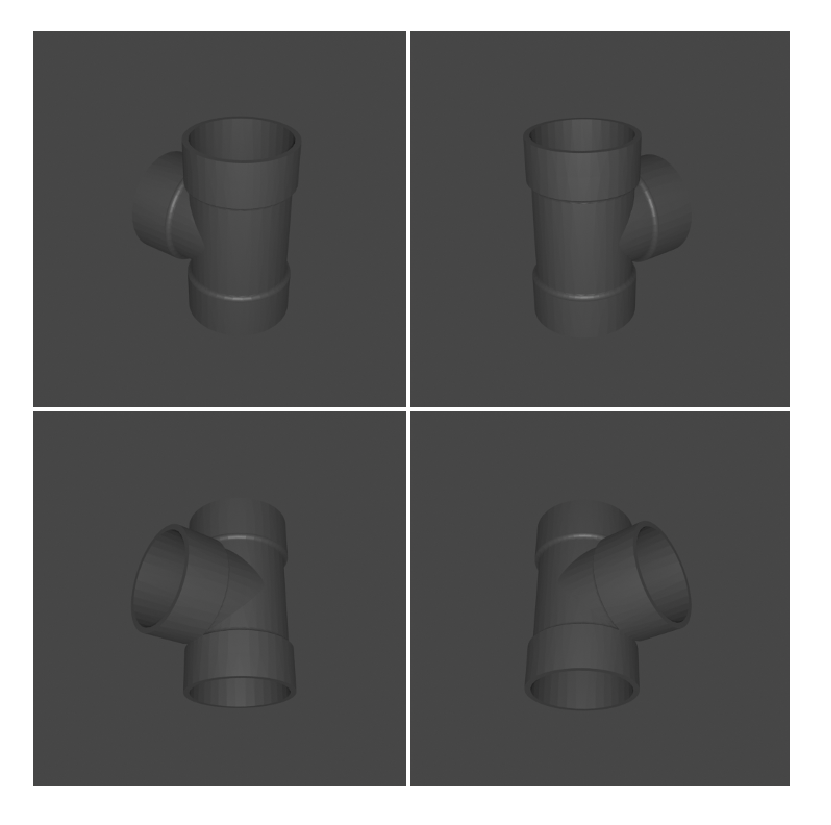
\includegraphics[height=85mm]{Figure/template.eps}
   \caption{テンプレート画像の例}
   \label{fig:f5}
\end{figure}

この際、ビューポイントは球状に分布させることで、対象物を全方向から均等に観察することができる。

こうして得られた複数の角度からの画像をテンプレートとして使用することで、対象物の姿勢推定や形状認識に必要な基準データが作成できる。
また、3Dモデルから点群データをopen3dのPythonライブラリを用いることで取得し、図\ref{fig:f6}に示す。
\begin{figure}[htbt]
  \centering
   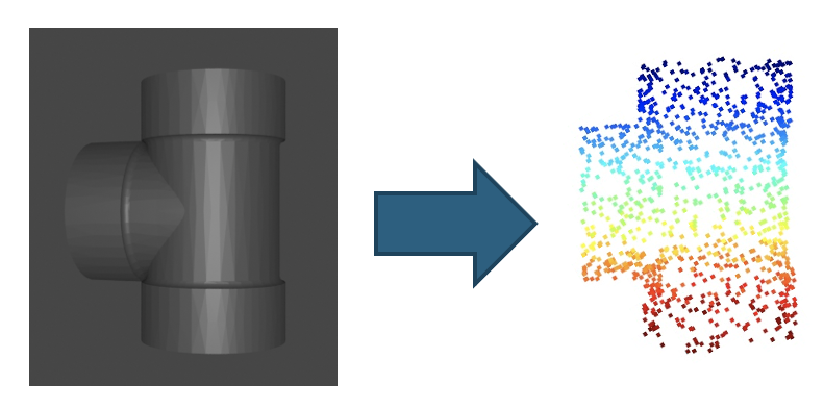
\includegraphics[height=55mm]{Figure/point_cloud.eps}
   \caption{3D点群データの例}
   \label{fig:f6}
\end{figure}

\section{評価指標}
6D姿勢推定の評価指標についてはADDとPrj-5を採用する[5]。

\begin{equation}
\textrm{ADD} = \frac{1}{\mathcal{M}}\sum_{\boldsymbol{x}\in \boldsymbol{\mathcal{M}}}||(\boldsymbol{\textrm{\textbf{Rx}}} + \boldsymbol{\textrm{\textbf{\textbf{T}}}}) - (\boldsymbol{\hat{\textrm{\textbf{Rx}}}} +  \boldsymbol{\hat{\textrm{\textbf{T}}}})||
\end{equation}

ADDについては、式(1)で示すように、推定された姿勢の3Dメッシュ頂点座標と、正解データの座標との平均距離を計算する。
ADDの評価基準では、推定された姿勢の平均距離がオブジェクトの直径の10%未満であれば、真とみなされる。
ここで、($\boldsymbol{\textrm{\textbf{R}}}$, $\boldsymbol{\textrm{\textbf{T}}}$)は真の姿勢と平行移動、 ($\boldsymbol{\hat{\textrm{\textbf{R}}}}$, $\boldsymbol{\hat{\textrm{\textbf{T}}}}$)は予測された回転と平行移動、$\boldsymbol{\mathcal{M}}$は3Dモデルの頂点集合である。

一方、Prj-5は、物体の3D点群を真の姿勢および推定された姿勢で2D画像上に射影した際の、各点間の2D距離の平均を計算する。
Prj-5の評価基準として、推定された姿勢の平均誤差が5ピクセル未満の場合、その推定姿勢を真と認定する。
これらの評価は全テスト画像に対して計算され、正確と判断された出力結果の割合をそれぞれADD-suc, Prj-5-sucとして示した。
従って、評価の値が高いほど、姿勢推定結果の精度が良いと考えられる。
さらに、各オブジェクトクラスの推定時間を計測し、推定の平均時間を算出した。
本研究では、配管データセットで670枚の画像から6D姿勢推定の評価を行った。


\section{結果と考察}
図4には6D姿勢推定の結果の一部が示し、表1には評価指標に基づくパフォーマンス結果がまとめられている。
結果には3Dバウンディングボックスで示された推定された姿勢を青色で、正解データの姿勢を緑色で表示されている。
これらが重なれば重なるほど、推定結果が正確であることを示す。
RGB画像に基づく6D姿勢推定の結果では示した画像2枚のように、曲管の推定結果が不正確であることが確認された。
曲管はT字管に比べて形状が複雑であり、カメラ視点の角度が急になると見えづらくなり姿勢が曲管の特徴を正確に捉えることが難しい。
一方、RGB-D画像に基づく6D姿勢推定の結果では、T字管および曲管の推定結果が良いことが確認された。
これは、RGB画像ベースでは使用していなかったDepth画像から点群データを姿勢推定に利用しているため、より配管の特徴を正確に捉えられたと考えられる。
また、表1において評価指標に基づくRGB-D画像ベースの6D姿勢推定の方が精度指標(ADD-suc、Prj-5-suc)においてRGB画像ベースよりも上回った。
一方で、処理時間に関してはRGB画像ベースの方が短い結果となった。
これは、Depth画像を使用していないため、処理時間が短縮されたと考えられる。
ただし、アイソメ図の作成においては、この処理時間の差は大きな影響を与えるものではないため、総合的にRGB-D画像ベースの6D姿勢推定の方が有効だと判断できる。

\begin{figure}[htbt]
	\centering
	\includegraphics[height=120mm]{Figure/compare_est.eps}
	\caption{6D姿勢推定の結果の一部}
	\label{fig:f2}
\end{figure}

\begin{table}[h]
	\centering
	\caption{評価指標に基づいた6D姿勢推定結果}
	\begin{tabular}{|p{1.7cm}|p{1.7cm}|p{1.7cm}|p{1.7cm}|}
	\hline
	& ADD-suc & Prj-5-suc & Time(s) \\
	\hline
	Gen6D & 0.443 & 0.697 & 0.178 \\
	\hline
	SAM-6D & 0.885 & 0.754 & 1.230 \\
	\hline
	\end{tabular}
\end{table}

続いて、アイソメ図生成の結果を図5に示し、正解データとの比較を図6に示す。

\begin{figure}[htbt]
	\centering
	\includegraphics[height=85mm]{Figure/result_iso_simple.eps}
	\caption{アイソメ図生成の結果}
	\label{fig:f2}
\end{figure}
\begin{figure}[htbt]
	\centering
	\includegraphics[height=85mm]{Figure/result_iso_simple_gt.eps}
	\caption{アイソメ図生成結果と正解データとの比較}
	\label{fig:f2}
\end{figure}

生成結果の色を青色で示し、正解データの色を赤色で示している。
RGB画像ベースの結果では、図3で示したように曲管の推定結果が不正確であることから向かい合うT字管と接続関係を正確に推定できなかった。
そのため、基準となるT字管からペアがみつからず地面や壁に設置されているものとして描画され、曲管部分が孤立してしまう結果となった。
ペアがない場合は固定値で長さを設定しているため、正解データとの比較ではT字管と曲管との線分に大きな差が生じてしまった。

一方、RGB-D画像ベースの結果では、T字管と曲管の接続関係を正確に推定できたため、アイソメ図の生成が可能であった。
接続関係にある配管ペアは線で結ばれ、2点間の座標の距離をもとに配管の長さを算出し、アイソメ図に描画した。
正解データとの比較では、図面同士が重なるように配置されていることが確認でき、RGB-D画像ベースの6D姿勢推定を用いたアイソメ図生成の有効性が示された。
